%=========================================================
% DM (Debug Module) Register
%=========================================================
\section{DM (Debug Module) Register}

The DM (Debug Module) registers are accessed by the DMI bus from the DTM. The address is specified by the DMI register according to the JTAG access.\\

\begin{table}[H]
    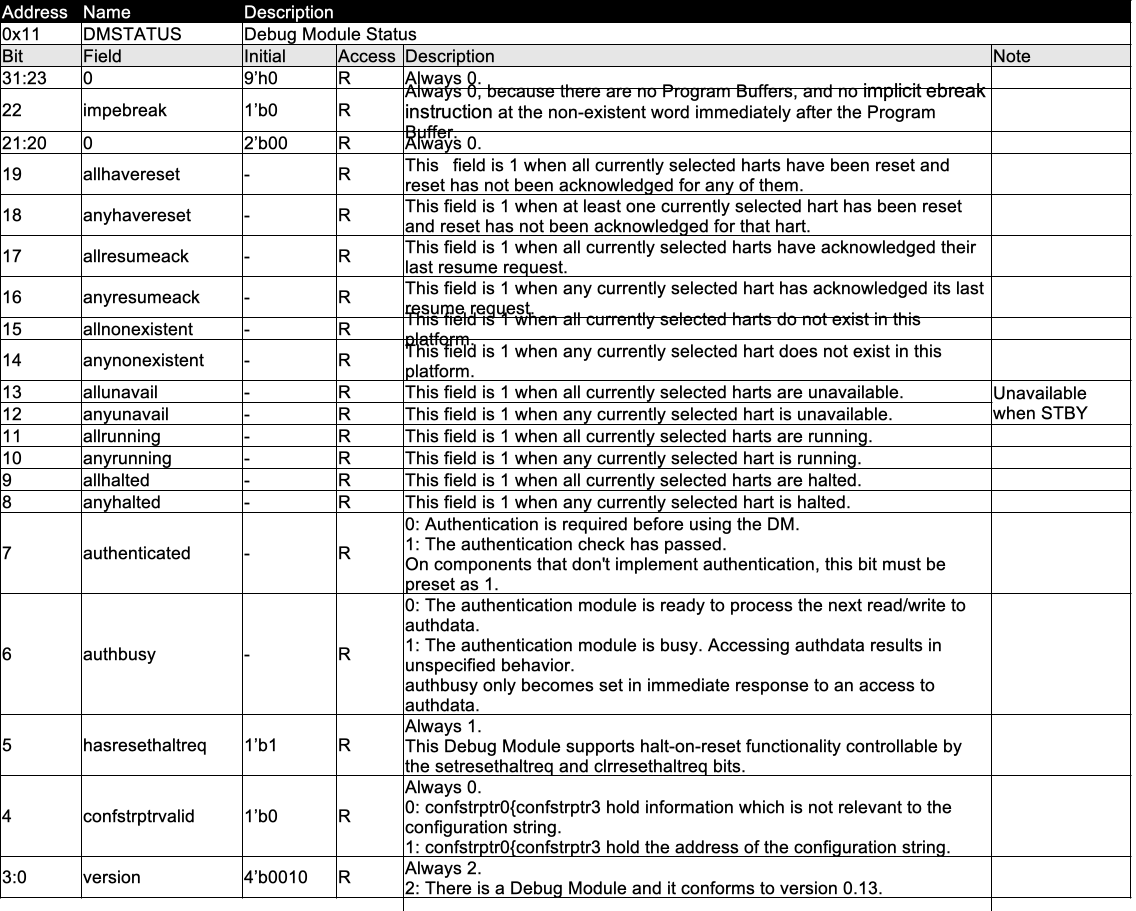
\includegraphics[width=1.00\columnwidth]{./Table/DMSTATUS.png}
    \caption{DMSTATUS}
    \label{tb:DMSTATUS}
\end{table}

\begin{table}[H]
    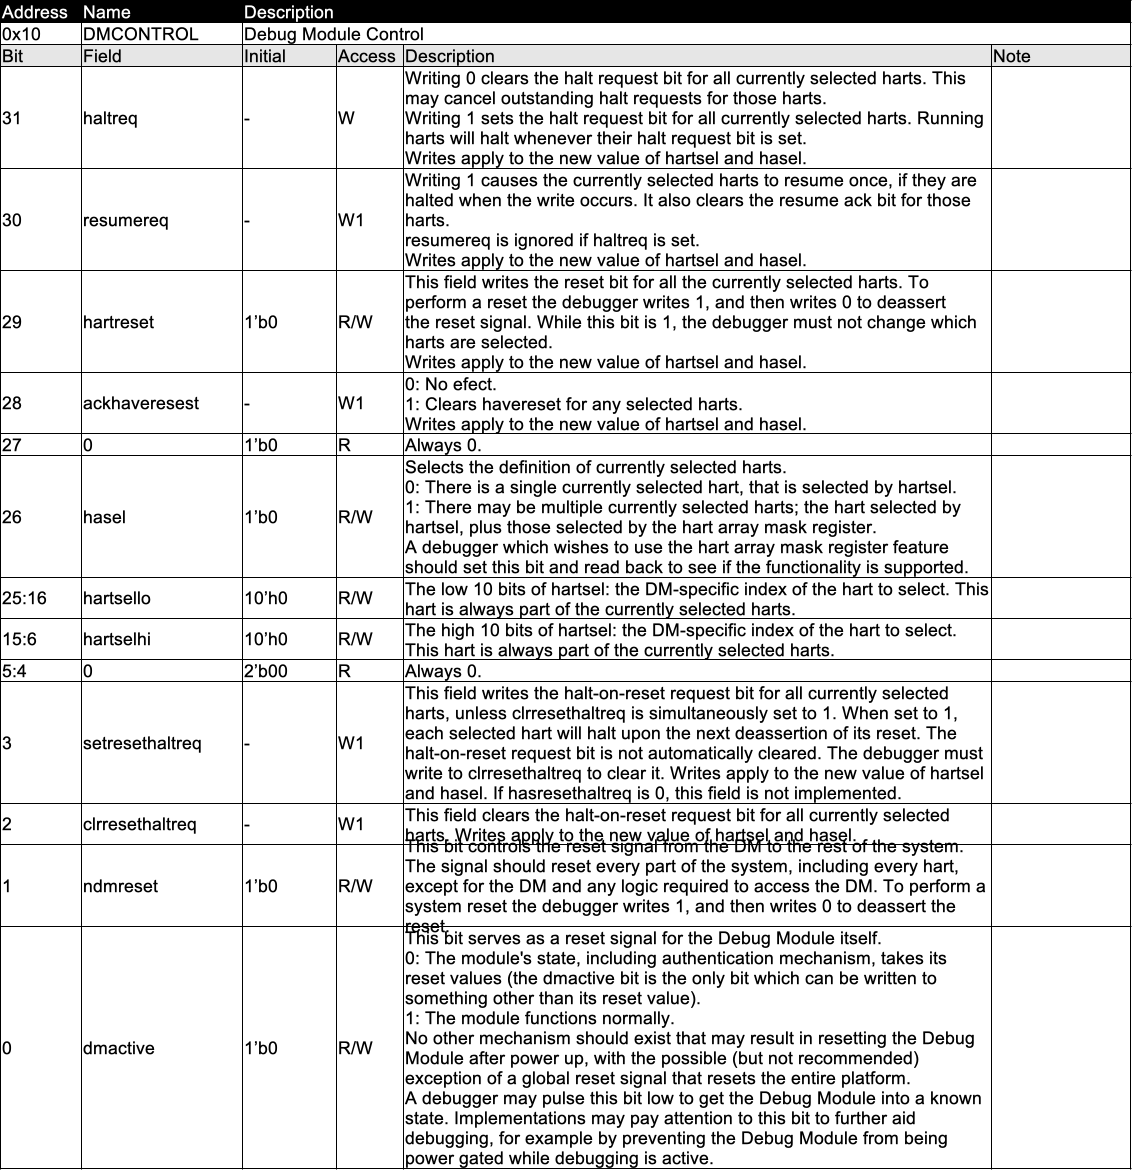
\includegraphics[width=1.00\columnwidth]{./Table/DMCONTROL.png}
    \caption{DMCONTROL}
    \label{tb:DMCONTROL}
\end{table}

\begin{table}[H]
    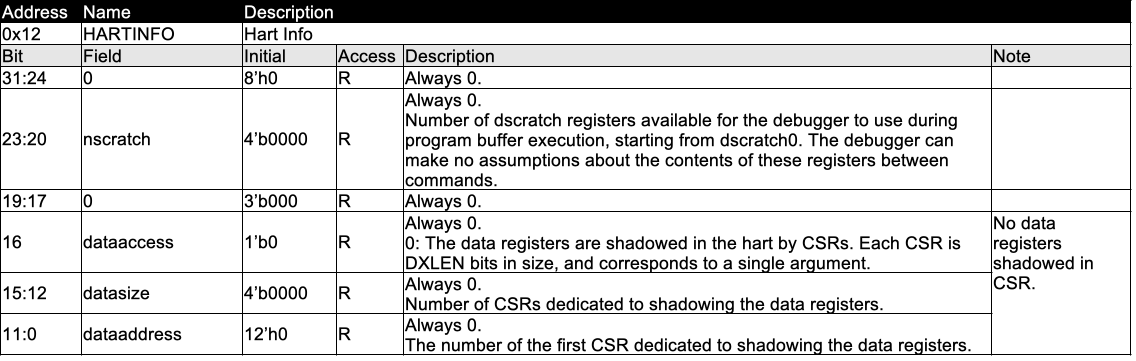
\includegraphics[width=1.00\columnwidth]{./Table/HARTINFO.png}
    \caption{HARTINFO}
    \label{tb:HARTINFO}
\end{table}

\begin{table}[H]
    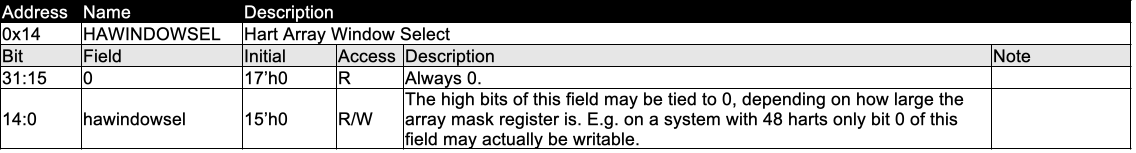
\includegraphics[width=1.00\columnwidth]{./Table/HAWINDOWSEL.png}
    \caption{HAWINDOWSEL}
    \label{tb:HAWINDOWSEL}
\end{table}

\begin{table}[H]
    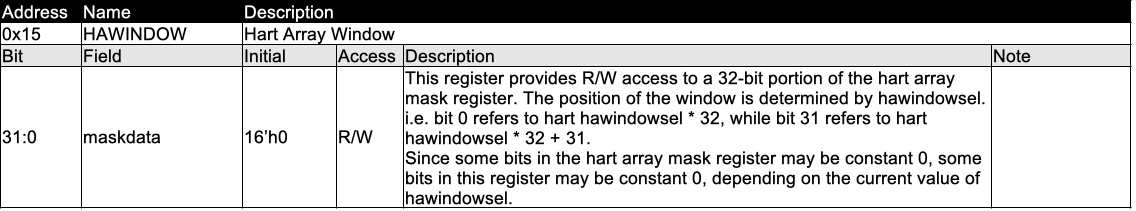
\includegraphics[width=1.00\columnwidth]{./Table/HAWINDOW.png}
    \caption{HAWINDOW}
    \label{tb:HAWINDOW}
\end{table}

\begin{table}[H]
    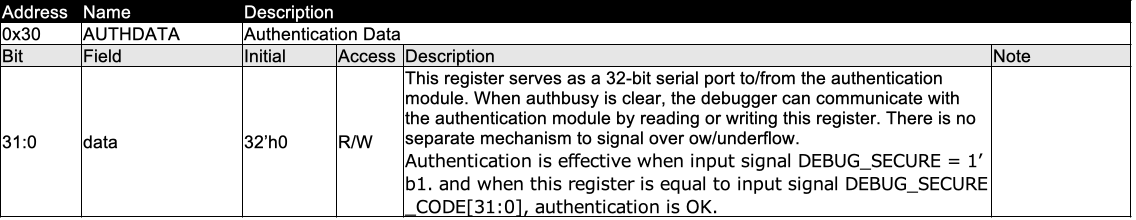
\includegraphics[width=1.00\columnwidth]{./Table/AUTHDATA.png}
    \caption{AUTHDATA}
    \label{tb:AUTHDATA}
\end{table}

\begin{table}[H]
    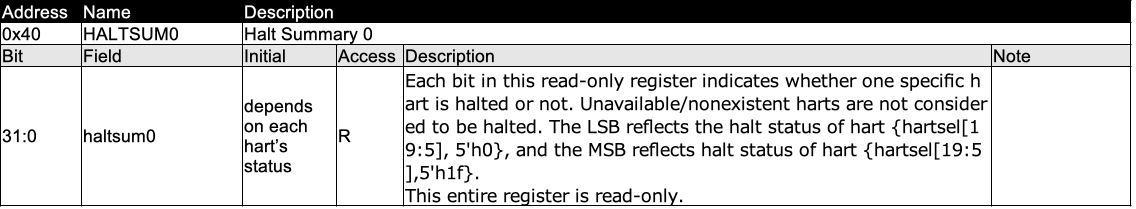
\includegraphics[width=1.00\columnwidth]{./Table/HALTSUM0.png}
    \caption{HALTSUM0}
    \label{tb:HALTSUM0}
\end{table}

\begin{table}[H]
    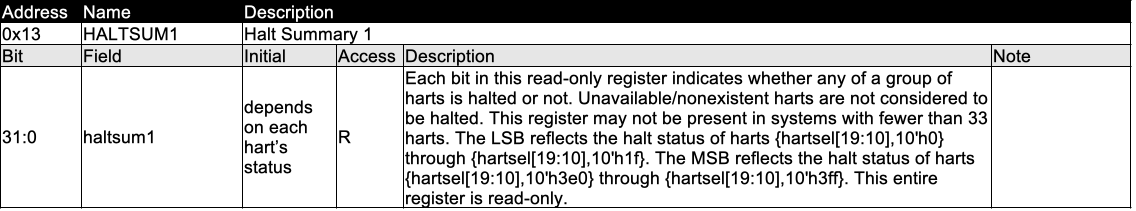
\includegraphics[width=1.00\columnwidth]{./Table/HALTSUM1.png}
    \caption{HALTSUM1}
    \label{tb:HALTSUM1}
\end{table}

\begin{table}[H]
    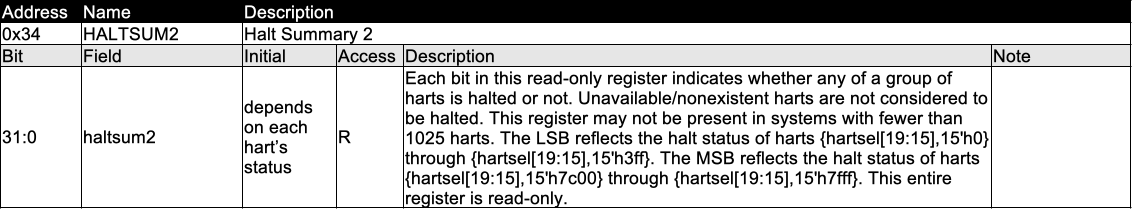
\includegraphics[width=1.00\columnwidth]{./Table/HALTSUM2.png}
    \caption{HALTSUM2}
    \label{tb:HALTSUM2}
\end{table}

\begin{table}[H]
    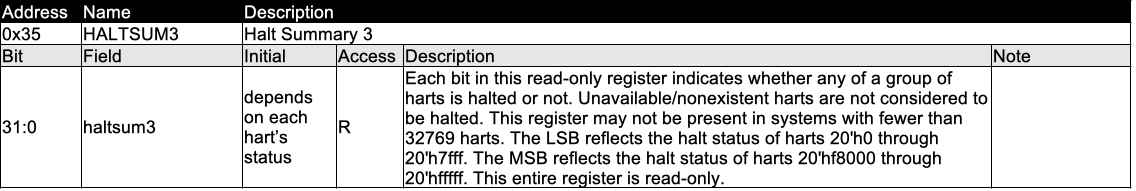
\includegraphics[width=1.00\columnwidth]{./Table/HALTSUM3.png}
    \caption{HALTSUM3}
    \label{tb:HALTSUM3}
\end{table}

